%\clearpage
%\twocolumn[
%    \begin{center}
%        \vspace{0.5cm} % Un poco de espacio arriba
%        \textbf{\LARGE ANEXOS} % Título grande y centrado
%        \vspace{0.5cm} % Espacio antes de que empiecen las columnas
%    \end{center}
%]
\clearpage
\twocolumn[
    \begin{center}
        \vspace{0.5cm} % A bit of space above
        \textbf{\LARGE APPENDICES} % Large centered title
        \vspace{0.5cm} % Space before columns start
    \end{center}
]

%\subsection*{Anexo A. Repositorio de Código y Reproducibilidad}
\subsection*{Appendix A. Code Repository and Reproducibility}

%Para garantizar la transparencia y replicabilidad de los experimentos, el código fuente completo, los pipelines de procesamiento y los scripts de entrenamiento se encuentran disponibles públicamente en:
To ensure transparency and replicability of the experiments, the complete source code, processing pipelines, and training scripts are publicly available at:

\begin{center}
    \texttt{https://github.com/amir1226/animaldet}
\end{center}

%El entorno de desarrollo utiliza el gestor de paquetes \texttt{uv} para manejar dependencias en conflicto mediante grupos aislados (\texttt{herdnet} y \texttt{rfdetr}), asegurando que cada arquitectura se ejecute con las versiones de bibliotecas exactas utilizadas durante la investigación.
The development environment uses the \texttt{uv} package manager to handle conflicting dependencies through isolated groups (\texttt{herdnet} and \texttt{rfdetr}), ensuring that each architecture runs with the exact library versions used during the research.

%\subsection*{Anexo B. Hiperparámetros y Configuración del Entrenamiento}
\subsection*{Appendix B. Hyperparameters and Training Configuration}

%Este anexo documenta los hiperparámetros y configuraciones utilizados durante el entrenamiento de los modelos HerdNet y RF-DETR (Nano, Small, Large). Todos los entrenamientos se ejecutaron en GPU NVIDIA A100 (80GB VRAM) utilizando PyTorch 2.x y CUDA 12.x.
This appendix documents the hyperparameters and configurations used during the training of HerdNet and RF-DETR (Nano, Small, Large) models. All training runs were executed on NVIDIA A100 GPU (80GB VRAM) using PyTorch 2.x and CUDA 12.x.

%\subsubsection*{B.1 HerdNet (Baseline)}
\subsubsection*{B.1 HerdNet (Baseline)}

%\paragraph{Fase 1 - Entrenamiento Inicial}
\paragraph{Phase 1 - Initial Training}
\begin{itemize}
%    \item \textbf{Épocas:} 100
    \item \textbf{Epochs:} 100
%    \item \textbf{Learning Rate Inicial:} $1 \times 10^{-4}$
    \item \textbf{Initial Learning Rate:} $1 \times 10^{-4}$
%    \item \textbf{Optimizador:} Adam
    \item \textbf{Optimizer:} Adam
%    \item \textbf{Weight Decay:} $5 \times 10^{-4}$
    \item \textbf{Weight Decay:} $5 \times 10^{-4}$
%    \item \textbf{Batch Size:} 4
    \item \textbf{Batch Size:} 4
%    \item \textbf{Learning Rate Schedule:} ReduceLROnPlateau
    \item \textbf{Learning Rate Schedule:} ReduceLROnPlateau
    \begin{itemize}
%        \item Mode: max (monitorea F1-Score)
        \item Mode: max (monitors F1-Score)
%        \item Patience: 10 épocas
        \item Patience: 10 epochs
%        \item Threshold: $1 \times 10^{-4}$
        \item Threshold: $1 \times 10^{-4}$
%        \item Cooldown: 10 épocas
        \item Cooldown: 10 epochs
%        \item Min LR: $1 \times 10^{-6}$
        \item Min LR: $1 \times 10^{-6}$
    \end{itemize}
%    \item \textbf{Tamaño de parche:} $512 \times 512$ píxeles
    \item \textbf{Patch Size:} $512 \times 512$ pixels
%    \item \textbf{Down Ratio:} 2 (para localización)
    \item \textbf{Down Ratio:} 2 (for localization)
%    \item \textbf{Warmup Iterations:} 100
    \item \textbf{Warmup Iterations:} 100
\end{itemize}

%\paragraph{Funciones de Pérdida (Fase 1)}
\paragraph{Loss Functions (Phase 1)}
\begin{itemize}
%    \item \textbf{Localización:} Focal Loss (reduction='mean', normalize=False)
    \item \textbf{Localization:} Focal Loss (reduction='mean', normalize=False)
%    \item \textbf{Clasificación:} Weighted Cross-Entropy Loss
    \item \textbf{Classification:} Weighted Cross-Entropy Loss
%    \item \textbf{Pesos por clase:} $w = [0.1, 1.0, 2.0, 1.0, 6.0, 12.0, 1.0]$
    \item \textbf{Class Weights:} $w = [0.1, 1.0, 2.0, 1.0, 6.0, 12.0, 1.0]$
\end{itemize}

%\paragraph{Fase 2 - Hard Negative Mining}
\paragraph{Phase 2 - Hard Negative Mining}
\begin{itemize}
%    \item \textbf{Épocas:} 50
    \item \textbf{Epochs:} 50
%    \item \textbf{Learning Rate Inicial:} $1 \times 10^{-6}$ (reducido 100×)
    \item \textbf{Initial Learning Rate:} $1 \times 10^{-6}$ (reduced 100×)
%    \item \textbf{Optimizador:} Adam
    \item \textbf{Optimizer:} Adam
%    \item \textbf{Weight Decay:} $5 \times 10^{-4}$
    \item \textbf{Weight Decay:} $5 \times 10^{-4}$
%    \item \textbf{Batch Size:} 4
    \item \textbf{Batch Size:} 4
%    \item \textbf{Warmup Iterations:} 1
    \item \textbf{Warmup Iterations:} 1
%    \item \textbf{Validation Frequency:} Cada 10 épocas
    \item \textbf{Validation Frequency:} Every 10 epochs
%    \item \textbf{Pesos por clase:} Idénticos a Fase 1
    \item \textbf{Class Weights:} Identical to Phase 1
%    \item \textbf{Checkpoint Inicial:} Mejor modelo de Fase 1 (selección por F1-Score máximo)
    \item \textbf{Initial Checkpoint:} Best Phase 1 model (selected by maximum F1-Score)
\end{itemize}

%\subsubsection*{B.2 RF-DETR (Todas las variantes)}
\subsubsection*{B.2 RF-DETR (All variants)}

%La Tabla \ref{tab:rfdetr_hyperparams} resume los hiperparámetros para las tres variantes de RF-DETR. Se destacan las diferencias en la resolución de entrada y la cantidad de parámetros.
Table \ref{tab:rfdetr_hyperparams} summarizes the hyperparameters for the three RF-DETR variants. The differences in input resolution and number of parameters are highlighted.

\begin{table}[htbp]
\centering
%\caption{Hiperparámetros de entrenamiento para RF-DETR (Nano, Small, Large).}
\caption{Training hyperparameters for RF-DETR (Nano, Small, Large).}
\label{tab:rfdetr_hyperparams}
\resizebox{\columnwidth}{!}{%
\begin{tabular}{lccc}
\hline
%\textbf{Parámetro} & \textbf{Nano} & \textbf{Small} & \textbf{Large} \\ \hline
\textbf{Parameter} & \textbf{Nano} & \textbf{Small} & \textbf{Large} \\ \hline
%\multicolumn{4}{l}{\textit{Arquitectura}} \\
\multicolumn{4}{l}{\textit{Architecture}} \\
%Tamaño de Entrada & $384 \times 384$ & $512 \times 512$ & $560 \times 560$ \\
Input Size & $384 \times 384$ & $512 \times 512$ & $560 \times 560$ \\
Backbone Base & DINOv2 & DINOv2 & DINOv2 \\
%Parámetros (aprox.) & \textbf{30.5 M} & \textbf{32.1 M} & \textbf{128 M} \\ \hline
Parameters (approx.) & \textbf{30.5 M} & \textbf{32.1 M} & \textbf{128 M} \\ \hline
%\multicolumn{4}{l}{\textit{Fase 1 - Entrenamiento Inicial}} \\
\multicolumn{4}{l}{\textit{Phase 1 - Initial Training}} \\
%Épocas & 50 & 50 & 50 \\
Epochs & 50 & 50 & 50 \\
Batch Size & 16 & 16 & 16 \\
Grad Accum Steps & 4 & 4 & 4 \\
%\textbf{Batch Efectivo} & \textbf{64} & \textbf{64} & \textbf{64} \\
\textbf{Effective Batch} & \textbf{64} & \textbf{64} & \textbf{64} \\
Learning Rate & Default* & Default* & Default* \\
%Optimizador & AdamW & AdamW & AdamW \\ \hline
Optimizer & AdamW & AdamW & AdamW \\ \hline
%\multicolumn{4}{l}{\textit{Fase 2 - Hard Negative Mining}} \\
\multicolumn{4}{l}{\textit{Phase 2 - Hard Negative Mining}} \\
%Épocas & 50 & 50 & 50 \\
Epochs & 50 & 50 & 50 \\
Batch Size & 2 & 2 & 2 \\
Grad Accum Steps & 8 & 8 & 8 \\
%\textbf{Batch Efectivo} & \textbf{16} & \textbf{16} & \textbf{16} \\
\textbf{Effective Batch} & \textbf{16} & \textbf{16} & \textbf{16} \\
Learning Rate (Decoder) & $1 \times 10^{-5}$ & $1 \times 10^{-5}$ & $1 \times 10^{-5}$ \\
Learning Rate (Encoder) & $1 \times 10^{-5}$ & $1 \times 10^{-5}$ & $1 \times 10^{-5}$ \\
Weight Decay & $1 \times 10^{-4}$ & $1 \times 10^{-4}$ & $1 \times 10^{-4}$ \\
EMA Decay & 0.993 & 0.993 & 0.993 \\
Multi-Scale Training & \checkmark & \checkmark & \checkmark \\
\hline
\end{tabular}%
}
\end{table}

%\textit{*Default: Learning rate con decaimiento por capas (layer-wise decay) según configuración estándar del framework RF-DETR $1 \times 10^{-4}$.}
\textit{*Default: Learning rate with layer-wise decay according to standard RF-DETR framework configuration $1 \times 10^{-4}$.}

\FloatBarrier

%\subsection*{Anexo C. Métricas Detalladas por Especie}
\subsection*{Appendix C. Detailed Metrics by Species}

%Este anexo presenta una desagregación completa de las métricas de rendimiento por especie para los cuatro modelos evaluados (HerdNet, RF-DETR Nano, RF-DETR Small, RF-DETR Large) en la Fase 2 del entrenamiento (con HNM). Las tablas permiten analizar el desempeño específico de cada arquitectura en el manejo de especies minoritarias y mayoritarias.
This appendix presents a complete breakdown of performance metrics by species for the four evaluated models (HerdNet, RF-DETR Nano, RF-DETR Small, RF-DETR Large) in Phase 2 of training (with HNM). The tables allow for analyzing the specific performance of each architecture in handling minority and majority species.

%\subsubsection*{C.1 Topi}
\subsubsection*{C.1 Topi}

%El Topi representa una de las especies mayoritarias del dataset (2.722 individuos, 26.6\% del total). La Tabla \ref{tab:metrics_topi} muestra que todos los modelos alcanzan un rendimiento elevado en esta especie, con F1-Scores superiores al 83\%.
The Topi represents one of the majority species in the dataset (2,722 individuals, 26.6\% of the total). Table \ref{tab:metrics_topi} shows that all models achieve high performance on this species, with F1-Scores exceeding 83\%.

\begin{table}[ht]
\centering
%\caption{Métricas de rendimiento para la especie Topi (Fase 2).}
\caption{Performance metrics for the Topi species (Phase 2).}
\label{tab:metrics_topi}
\resizebox{\columnwidth}{!}{%
\begin{tabular}{lcccc}
\hline
%\textbf{Métrica} & \textbf{HerdNet} & \textbf{RF-DETR Nano} & \textbf{RF-DETR Small} & \textbf{RF-DETR Large} \\ \hline
\textbf{Metric} & \textbf{HerdNet} & \textbf{RF-DETR Nano} & \textbf{RF-DETR Small} & \textbf{RF-DETR Large} \\ \hline
F1-Score & 0.8559 & 0.8381 & \textbf{0.8960} & 0.8550 \\
Precision & 0.8371 & 0.7615 & \textbf{0.8800} & 0.7909 \\
Recall & 0.8756 & 0.9319 & 0.9126 & \textbf{0.9304} \\
MAE & 1.7042 & 2.1059 & \textbf{1.5735} & 1.9615 \\
RMSE & 2.8009 & 3.4007 & \textbf{2.9180} & 3.3722 \\ \hline
\end{tabular}%
}
\end{table}

%\subsubsection*{C.2 Búfalo}
\subsubsection*{C.2 Buffalo}

%El Búfalo es otra especie mayoritaria del dataset (1.509 individuos, 14.7\% del total). La Tabla \ref{tab:metrics_buffalo} revela un patrón de rendimiento similar al Topi, con mejoras consistentes de RF-DETR Small.
The Buffalo is another majority species in the dataset (1,509 individuals, 14.7\% of the total). Table \ref{tab:metrics_buffalo} reveals a performance pattern similar to Topi, with consistent improvements from RF-DETR Small.

\begin{table}[ht]
\centering
%\caption{Métricas de rendimiento para la especie Búfalo (Fase 2).}
\caption{Performance metrics for the Buffalo species (Phase 2).}
\label{tab:metrics_buffalo}
\resizebox{\columnwidth}{!}{%
\begin{tabular}{lcccc}
\hline
%\textbf{Métrica} & \textbf{HerdNet} & \textbf{RF-DETR Nano} & \textbf{RF-DETR Small} & \textbf{RF-DETR Large} \\ \hline
\textbf{Metric} & \textbf{HerdNet} & \textbf{RF-DETR Nano} & \textbf{RF-DETR Small} & \textbf{RF-DETR Large} \\ \hline
F1-Score & 0.8115 & 0.8024 & \textbf{0.8435} & 0.8313 \\
Precision & 0.9170 & 0.8471 & \textbf{0.9531} & 0.8944 \\
Recall & 0.7278 & 0.7622 & 0.7564 & \textbf{0.7765} \\
MAE & 3.5000 & 3.1786 & 3.3333 & \textbf{3.0400} \\
RMSE & 5.9702 & 6.2593 & 6.4936 & \textbf{5.9464} \\ \hline
\end{tabular}%
}
\end{table}

%\subsubsection*{C.3 Kob}
\subsubsection*{C.3 Kob}

%El Kob es una especie mayoritaria del dataset (2.370 individuos, 23.1\% del total). La Tabla \ref{tab:metrics_kob} muestra un rendimiento excepcional de RF-DETR Small.
The Kob is a majority species in the dataset (2,370 individuals, 23.1\% of the total). Table \ref{tab:metrics_kob} shows exceptional performance from RF-DETR Small.

\begin{table}[ht]
\centering
%\caption{Métricas de rendimiento para la especie Kob (Fase 2).}
\caption{Performance metrics for the Kob species (Phase 2).}
\label{tab:metrics_kob}
\resizebox{\columnwidth}{!}{%
\begin{tabular}{lcccc}
\hline
%\textbf{Métrica} & \textbf{HerdNet} & \textbf{RF-DETR Nano} & \textbf{RF-DETR Small} & \textbf{RF-DETR Large} \\ \hline
\textbf{Metric} & \textbf{HerdNet} & \textbf{RF-DETR Nano} & \textbf{RF-DETR Small} & \textbf{RF-DETR Large} \\ \hline
F1-Score & 0.8751 & 0.8156 & \textbf{0.9051} & 0.8019 \\
Precision & 0.8484 & 0.7812 & \textbf{0.9432} & 0.9029 \\
Recall & \textbf{0.9036} & 0.8532 & 0.8700 & 0.7212 \\
MAE & 1.0283 & 1.2952 & \textbf{0.6915} & 1.5506 \\
RMSE & 1.9882 & 2.1647 & \textbf{1.8072} & 3.2568 \\ \hline
\end{tabular}%
}
\end{table}


%\subsubsection*{C.4 Facóquero}
\subsubsection*{C.4 Warthog}

%El Facóquero es una especie minoritaria del dataset (433 individuos, 4.2\% del total). La Tabla \ref{tab:metrics_warthog} revela uno de los desafíos más significativos del estudio: todos los modelos presentan un rendimiento limitado en esta clase.
The Warthog is a minority species in the dataset (433 individuals, 4.2\% of the total). Table \ref{tab:metrics_warthog} reveals one of the most significant challenges of the study: all models exhibit limited performance on this class.

\begin{table}[ht]
\centering
%\caption{Métricas de rendimiento para la especie Facóquero (Fase 2).}
\caption{Performance metrics for the Warthog species (Phase 2).}
\label{tab:metrics_warthog}
\resizebox{\columnwidth}{!}{%
\begin{tabular}{lcccc}
\hline
%\textbf{Métrica} & \textbf{HerdNet} & \textbf{RF-DETR Nano} & \textbf{RF-DETR Small} & \textbf{RF-DETR Large} \\ \hline
\textbf{Metric} & \textbf{HerdNet} & \textbf{RF-DETR Nano} & \textbf{RF-DETR Small} & \textbf{RF-DETR Large} \\ \hline
F1-Score & 0.4151 & 0.3788 & 0.4065 & \textbf{0.4493} \\
Precision & 0.3882 & 0.4310 & 0.5102 & \textbf{0.4844} \\
Recall & \textbf{0.4459} & \textbf{0.3378} & \textbf{0.3378} & \textbf{0.4189} \\
MAE & 2.2432 & 2.4667 & 2.4815 & \textbf{2.4000} \\
RMSE & \textbf{3.1322} & 3.5496 & 3.5013 & 3.4351 \\ \hline
\end{tabular}%
}
\end{table}

%\subsubsection*{C.5 Cobo de agua}
\subsubsection*{C.5 Waterbuck}

%El Cobo de agua es la especie más minoritaria del dataset (241 individuos, 2.4\% del total). La Tabla \ref{tab:metrics_waterbuck} muestra el impacto más pronunciado de las arquitecturas basadas en Transformers.
The Waterbuck is the most minority species in the dataset (241 individuals, 2.4\% of the total). Table \ref{tab:metrics_waterbuck} shows the most pronounced impact of Transformer-based architectures.

\begin{table}[ht]
\centering
%\caption{Métricas de rendimiento para la especie Cobo de agua (Fase 2).}
\caption{Performance metrics for the Waterbuck species (Phase 2).}
\label{tab:metrics_waterbuck}
\resizebox{\columnwidth}{!}{%
\begin{tabular}{lcccc}
\hline
%\textbf{Métrica} & \textbf{HerdNet} & \textbf{RF-DETR Nano} & \textbf{RF-DETR Small} & \textbf{RF-DETR Large} \\ \hline
\textbf{Metric} & \textbf{HerdNet} & \textbf{RF-DETR Nano} & \textbf{RF-DETR Small} & \textbf{RF-DETR Large} \\ \hline
F1-Score & 0.6849 & 0.6237 & 0.7097 & \textbf{0.8158} \\
Precision & 0.6757 & 0.5088 & 0.8462 & \textbf{0.7750} \\
Recall & 0.6944 & \textbf{0.8056} & 0.6111 & \textbf{0.8611} \\
MAE & 1.2500 & 1.4375 & 2.5714 & \textbf{1.2000} \\
RMSE & 1.5000 & 2.2500 & 3.0237 & \textbf{1.4142} \\ \hline
\end{tabular}%
}
\end{table}

%\subsubsection*{C.6 Elefante}
\subsubsection*{C.6 Elephant}

%El Elefante es la especie más numerosa del dataset (2.964 individuos, 28.9\% del total). La Tabla \ref{tab:metrics_elephant} revela el fallo de RF-DETR Nano en esta clase.
The Elephant is the most numerous species in the dataset (2,964 individuals, 28.9\% of the total). Table \ref{tab:metrics_elephant} reveals the failure of RF-DETR Nano on this class.

\begin{table}[ht]
\centering
%\caption{Métricas de rendimiento para la especie Elefante (Fase 2).}
\caption{Performance metrics for the Elephant species (Phase 2).}
\label{tab:metrics_elephant}
\resizebox{\columnwidth}{!}{%
\begin{tabular}{lcccc}
\hline
%\textbf{Métrica} & \textbf{HerdNet} & \textbf{RF-DETR Nano} & \textbf{RF-DETR Small} & \textbf{RF-DETR Large} \\ \hline
\textbf{Metric} & \textbf{HerdNet} & \textbf{RF-DETR Nano} & \textbf{RF-DETR Small} & \textbf{RF-DETR Large} \\ \hline
F1-Score & 0.6956 & 0.0363 & 0.8649 & \textbf{0.8641} \\
Precision & 0.6707 & 0.4483 & 0.8995 & \textbf{0.8549} \\
Recall & 0.7224 & 0.0189 & 0.8328 & \textbf{0.8735} \\
MAE & 2.5728 & 6.5900 & \textbf{1.0700} & 1.2300 \\
RMSE & 4.4142 & 10.3068 & \textbf{1.5969} & 3.9154 \\ \hline
\end{tabular}%
}
\end{table}

\FloatBarrier

%\subsection*{Anexo D. Ejemplos Cualitativos Adicionales}
\subsection*{Appendix D. Additional Qualitative Examples}

%A continuación, la Figura \ref{fig:anexo_c_1} ilustra los resultados de detección para el Cobo de agua. Esta comparación cualitativa sobre 4 individuos permite visualizar el desempeño de los modelos en una de las especies con menor representación (minoritaria) en el conjunto de entrenamiento.
The following Figure \ref{fig:anexo_c_1} illustrates the detection results for the Waterbuck. This qualitative comparison on 4 individuals allows visualizing the performance of the models on one of the species with the least representation (minority) in the training set.
\begin{figure}[ht]
    \centering
    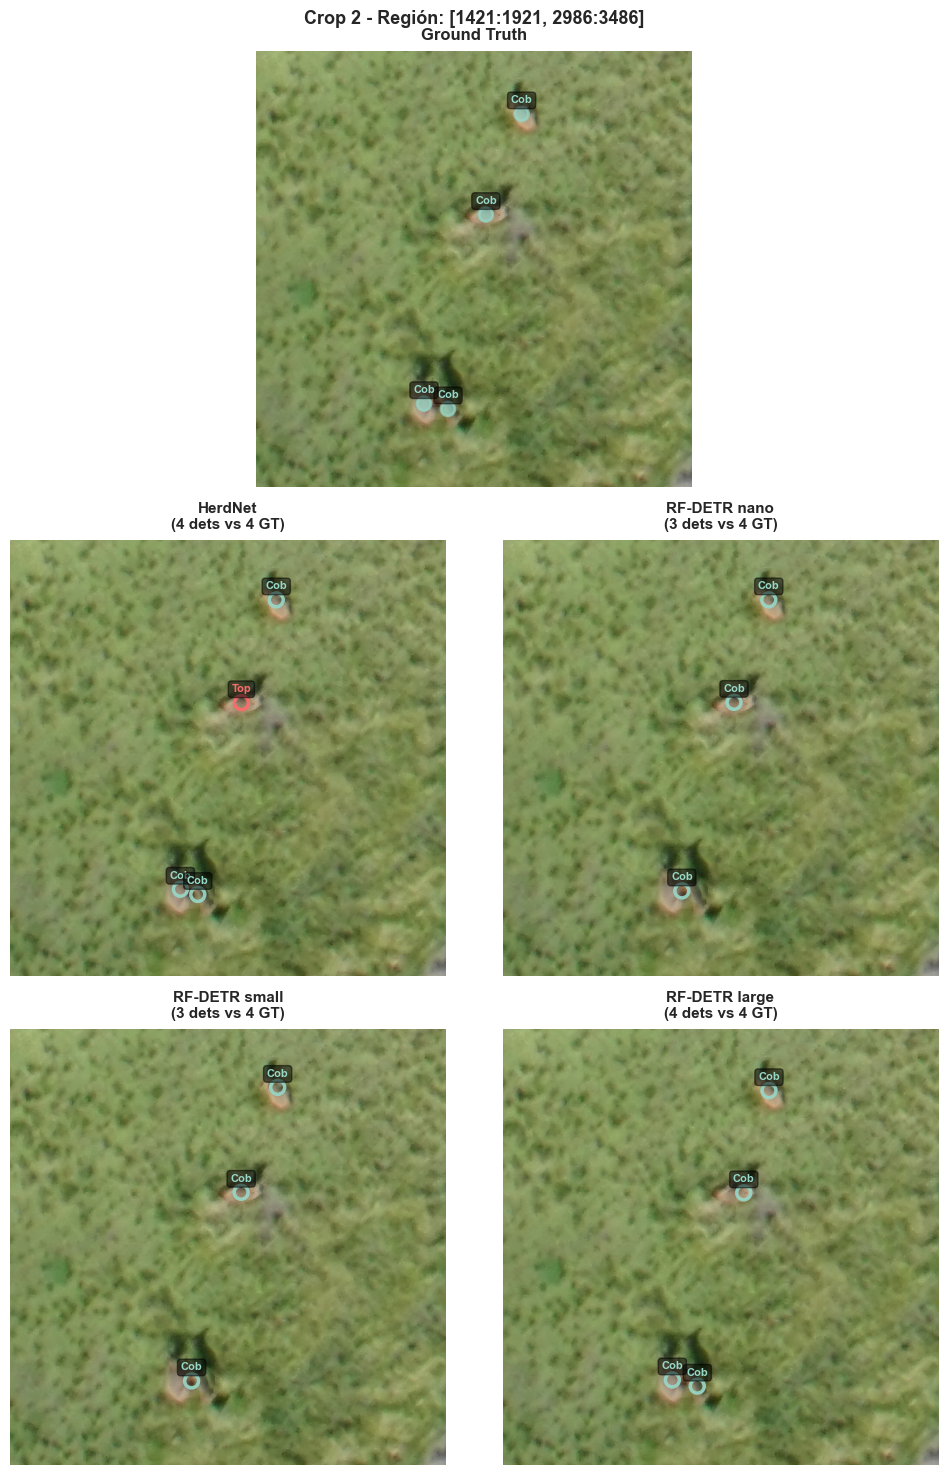
\includegraphics[width=0.9\columnwidth, height=1.78\columnwidth]{static/img/anexo_c_comp_1.png}
%    \caption{Comparación cualitativa del cobo de agua. Se observan 4 cobos de agua.}
    \caption{Qualitative comparison of the waterbuck. 4 waterbucks are observed.}
    \label{fig:anexo_c_1}
\end{figure}

\FloatBarrier
%La Figura \ref{fig:anexo_c_2} presenta un escenario con 2 individuos de la especie Topi. Esta comparación sirve para evaluar la precisión de clasificación y localización en una de las especies de antílopes más frecuentes y de tamaño medio del conjunto de datos.
Figure \ref{fig:anexo_c_2} presents a scenario with 2 individuals of the Topi species. This comparison serves to evaluate the classification and localization accuracy on one of the most frequent medium-sized antelope species in the dataset.

\begin{figure}[ht]
    \centering
    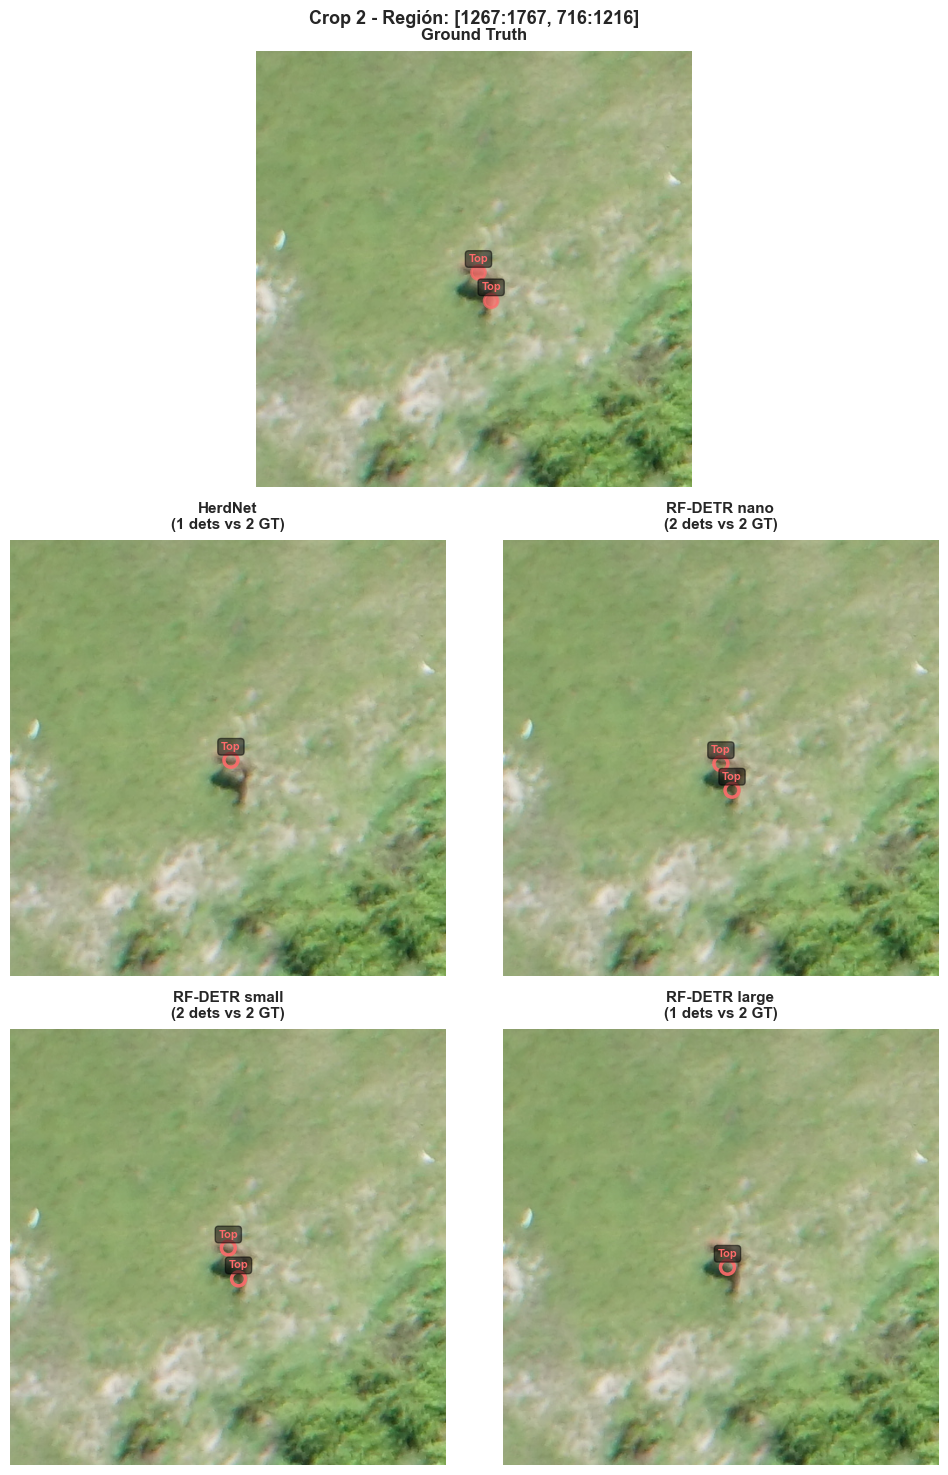
\includegraphics[width=0.9\columnwidth, height=2.25\columnwidth]{static/img/anexo_c_comp_2.png}
%    \caption{Comparación cualitativa del topi. Se observan 2 topis.}
    \caption{Qualitative comparison of the topi. 2 topis are observed.}
    \label{fig:anexo_c_2}
\end{figure}
\FloatBarrier
%En la siguiente Figura \ref{fig:anexo_c_3} se visualizan los resultados para el Facóquero. Este ejemplo con 3 individuos es crítico para analizar la capacidad de los diferentes modelos para detectar objetivos de tamaño muy pequeño, un desafío donde suelen ocurrir omisiones (falsos negativos).
In the following Figure \ref{fig:anexo_c_3} the results for the Warthog are visualized. This example with 3 individuals is critical for analyzing the capability of the different models to detect very small-sized targets, a challenge where omissions (false negatives) often occur.

\begin{figure}[ht]
    \centering
    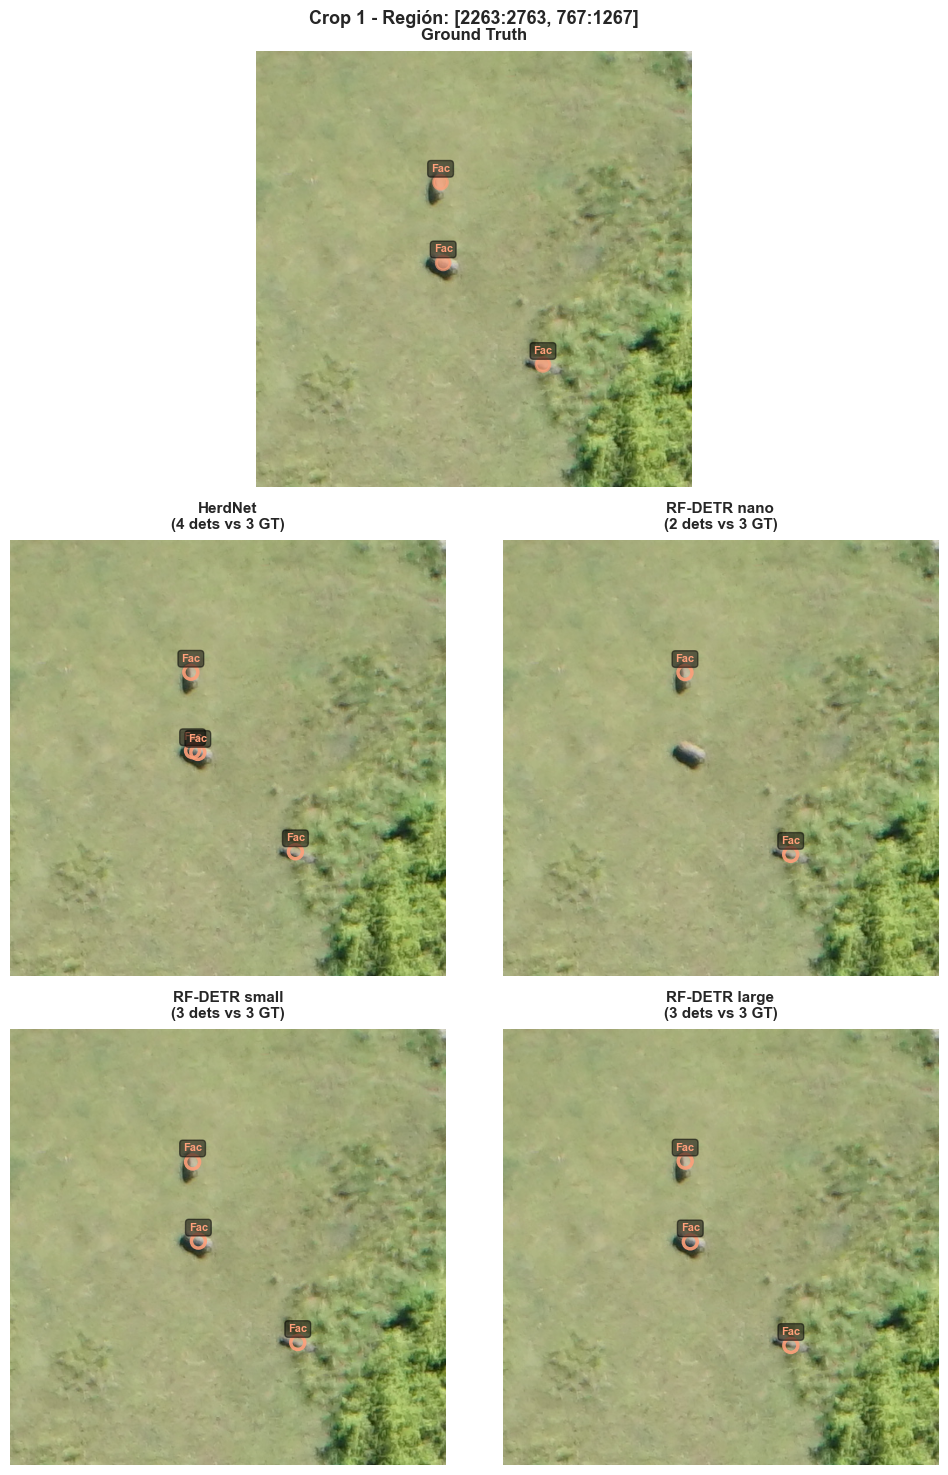
\includegraphics[width=0.9\columnwidth, height=2.25\columnwidth]{static/img/anexo_c_comp_3.png}
%    \caption{Comparación cualitativa del Facóquero. Se observan 2 facóqueros.}
    \caption{Qualitative comparison of the Warthog. 2 warthogs are observed.}
    \label{fig:anexo_c_3}
\end{figure}
\FloatBarrier
%Por último, la Figura \ref{fig:anexo_c_4} presenta una comparación cualitativa sobre un grupo de 6 Búfalos. Este escenario permite observar el comportamiento de los detectores ante una especie de gran tamaño, coloración oscura y morfología distintiva.
Finally, Figure \ref{fig:anexo_c_4} presents a qualitative comparison on a group of 6 Buffalos. This scenario allows observing the behavior of the detectors when faced with a large-sized species with dark coloration and distinctive morphology.

\begin{figure}[ht]
    \centering
    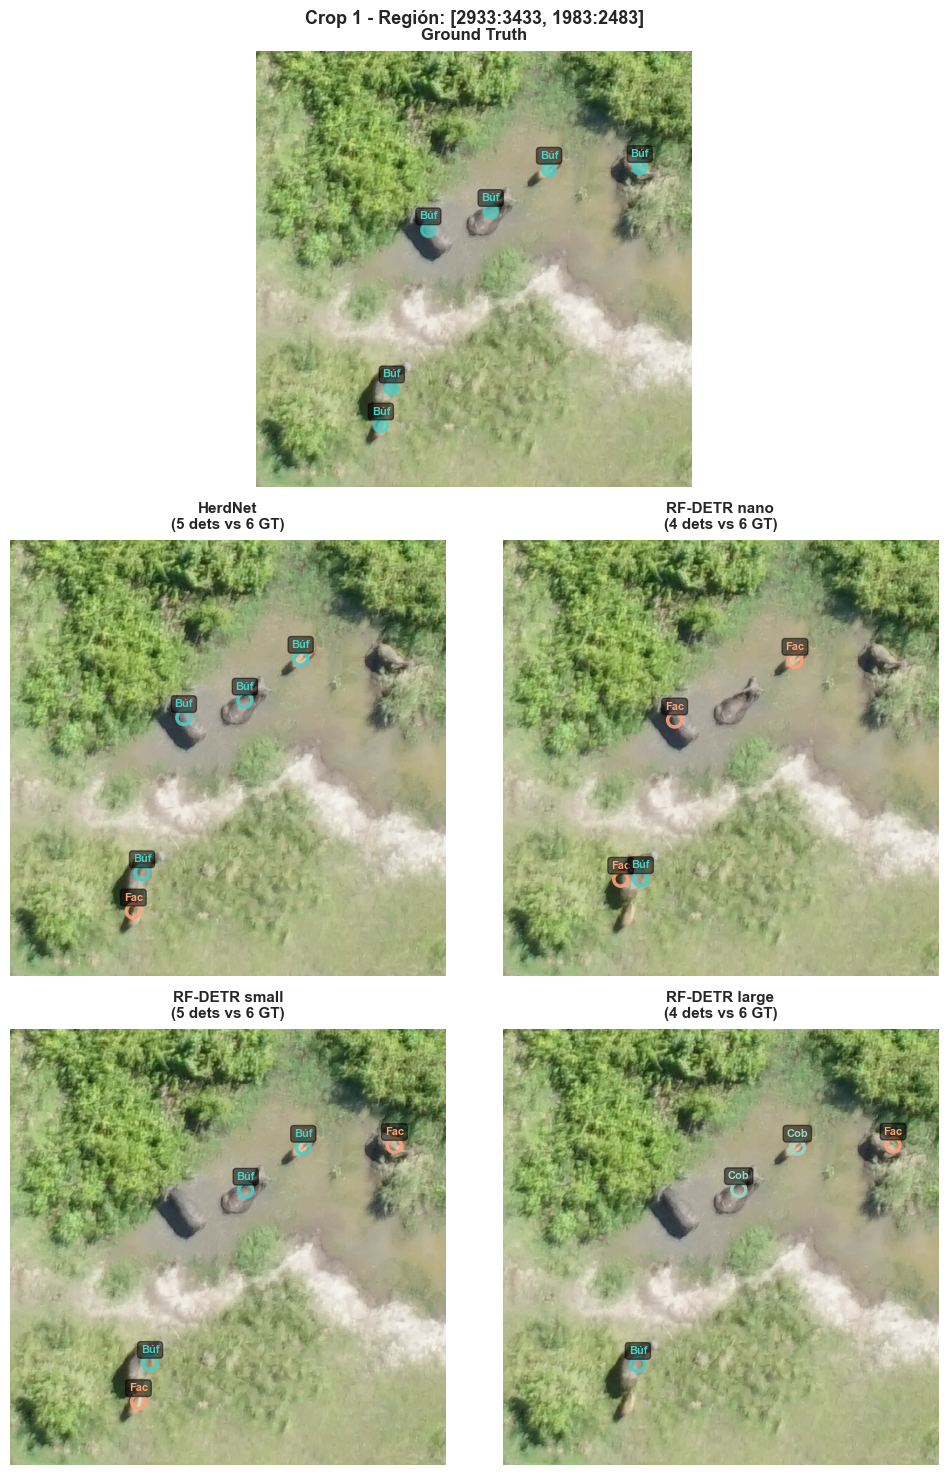
\includegraphics[width=0.9\columnwidth, height=2.25\columnwidth]{static/img/anexo_c_comp_4.png}
%    \caption{Comparación cualitativa del Búfalo. Se observan 6 búfalos.}
    \caption{Qualitative comparison of the Buffalo. 6 buffalos are observed.}
    \label{fig:anexo_c_4}
\end{figure}
